\documentclass[xcolor=dvipsnames]{beamer} %,compress,handout
\mode<presentation>
{
	\usetheme{Copenhagen}
	\usefonttheme{professionalfonts}
	\useoutertheme[footline=authortitle,subsection=false]{miniframes}
}

\setbeamertemplate{frametitle}{%
	\nointerlineskip%
	\begin{beamercolorbox}[wd=\paperwidth,ht=2.5ex,dp=1ex]{frametitle}
		\hspace*{1ex}\insertframetitle%
	\end{beamercolorbox}%
}

\setbeamertemplate{frametitle continuation}[from second][]
% setting for frame breaks

\newcounter{sauvegardeenumi}
\newcommand{\estop}{\setcounter{sauvegardeenumi}{\theenumi}}
\newcommand{\estart}{\setcounter{enumi}{\thesauvegardeenumi}}
% new counter for multi-frame enumeration

\setbeamercovered{transparent}
\setbeamercolor{bgcyan}{fg=black,bg=cyan}
\setbeamercolor{bggreen}{fg=black,bg=green}
\setbeamercolor{bgred}{fg=black,bg=red}

\makeatletter
\renewcommand\eqref[1]{%
	\textup{\usebeamercolor[fg]{structure}\tagform@{\ref{#1}}}%
}
%eqref colors
%\usepackage{calrsfs} % curly fonts, \mathcal
%\usepackage{mtpro2}
\usepackage[cal=rsfs,scr=euler]{mathalfa}
%\usepackage{enumitem} % redefine enumerate
\usepackage{tabularx}
\usepackage{graphicx} % include graphs

\usepackage{colortbl,amsmath,amssymb}
\usepackage[UTF8]{ctex}
\usepackage{textpos} % add logo
%\logo{\includegraphics[height=0.5cm]{./pic/bit_logo} %add logo
\usepackage{tensor} % manipulate tensor
\hypersetup{pdfpagemode=FullScreen} % full-screen when viewing the pdf

\usepackage[most]{tcolorbox} % equation array box

%%%%%%%%%%%%%%%%%%%%%%%%%%%%%%%%%%%%%%%%%%%%%%%%%%%%%%%%%%%%%%%%%%%%%%%%%%%%%%%%
% newcommand % 
%%%%%%%%%%%%%%%%%%%%%%%%%%%%%%%%%%%%%%%%%%%%%%%%%%%%%%%%%%%%%%%%%%%%%%%%%%%%%%%%
\newcommand{\newc}{\newcommand*}
\newc{\nc}{\newc}
\newc{\be}{\begin{equation}}
\newc{\ee}{\end{equation}}
\newc{\bea}{\begin{eqnarray}}
\newc{\eea}{\end{eqnarray}}
\newc{\bear}{\begin{eqnarray}}
\newc{\eear}{\end{eqnarray}}
\newc{\kp}{\kappa}
\newc{\p}{\partial}
\newc{\om}{\omega}
\newc{\Om}{\Omega}
\newc{\mc}{\mathcal}
\newc{\ms}{\mathscr}
\newc{\s}{\sigma}
\newc{\ts}{\tensor}
\newc{\g}{\gamma}
\newc{\Ga}{\Gamma}
\newc{\al}{\alpha}
\newc{\bt}{\beta}
\newc{\la}{\lambda}
\newc{\dt}{\delta}
\newc{\dH}{\dot{H}}
\newc{\dphi}{\dot{\phi}}
\newc{\es}{\epsilon}
\newc{\tH}{\tilde{h}}
\newc{\La}{\Lambda}
\newc{\mb}{\mathbf} 
\newc{\ie}{{\it i.e.} }
\newc{\eg}{{\it e.g.} }
\newc{\etc}{{\it etc.} }
\newc{\etal}{{\it et al.}}
\newc{\lcdm}{$\Lambda$CDM}
\newc{\sqrtg}{\sqrt{- g}}
\newc{\mf}{\mathfrak}
\newc{\gtg}{\mf{g}} %gothic g
\newc{\bp}{\mathbf{p}}
\newc{\fs}{{\rm{\it f\sigma_8}}}
\newc{\D}{\partial}
\newc{\td}{\tilde}
\newc{\nb}{\nabla}
\newc{\vp}{\varphi}
\newc{\Gac}{{\stackrel{\circ}{\Gamma}}}
\newc{\nac}{{\stackrel{\circ}{\nabla}}}
\newc{\Rc}{{\stackrel{\circ}{R}}}
\newc{\ra}{\rightarrow}
\newc{\Ra}{\Rightarrow}
\newc{\lra}{\leftrightarrow}
\newc{\Lra}{\Leftrightarrow}
\newc{\so}{\therefore}
\newc{\lap}{\mathop{}\!\mathbin\bigtriangleup} %Laplace
\newc{\dl}{\mathop{}\!\mathbin\Box} %DAlambert
\newc{\hf}{\frac{1}{2}}
\newc{\lvc}{LIGO/Virgo}
\nc{\Msun}{M_\odot}  
\nc{\fpbh}{f_{\mathrm{pbh}}}
%%%%%%%%%%%%%%%%%%%%%%%%%%%%%%%%%%%%%%%%%%%%%%%%%%%%%%%%%%%%%%%%%%%%%%%%%%%%%%%%
% %only used in this tex file %
\newc{\red}[1]{\textcolor{red}{#1}}
\newc{\cyan}[1]{\textcolor{cyan}{#1}}
\newc{\green}[1]{\textcolor{green}{#1}}
\newc{\blue}[1]{\textcolor{blue}{#1}}
\newc{\re}[1]{\emph{\textcolor{red}{#1}}}

\nc{\rd}{\mathrm{d}}

\def\({\left(}
\def\){\right)}
\nc{\vth}{\vec{\theta}}
\nc{\rmd}{\mathrm{d}}
\nc{\vd}{\vec{d}}
\nc{\vla}{\vec{\lambda}}

%%%%%%%%%%%%%%%%%%%%%%%%%%%%%%%%%%%%%%%%%%%%%%%%%%%%%%%%%%%%%%%%%%%%%%%%%%%%%%%%
%\AtBeginSection[]
%  {
%     \begin{frame}<beamer>
%     \frametitle{Outline}
%            \tableofcontents[currentsection]
%     \end{frame}
%  }
%show a plan before every section

%%%%%%%%%%%%%%%%%%%%%%%%%%%%%%%%%%%%%%%%%%%%%%%%%%%%%%%%%%%%%%%%%%%%%%%%%%%%%%%%
\begin{document}

\kaishu
\setbeamertemplate{footline}
{%
	\begin{beamercolorbox}[colsep=1.5pt]{upper separation line foot}
    \end{beamercolorbox}
    \begin{beamercolorbox}[ht=2.5ex,dp=1.125ex,%
      leftskip=.3cm,rightskip=.3cm plus1fil]{title in head/foot}%
      \leavevmode{\usebeamerfont{title in head/foot}\insertshortauthor}%
      \hfill%
      {\usebeamerfont{author in head/foot}\usebeamercolor[fg]{author in head/foot}\insertshorttitle}%
      \hfill%
      {\usebeamerfont{date in head/foot}\usebeamercolor[fg]{date in head/foot}\insertshortdate}%
    \end{beamercolorbox}%
    \begin{beamercolorbox}[colsep=1.5pt]{lower separation line foot}
    \end{beamercolorbox}
}



%%%%%%%%%%%%%%%%%%%%%%%%%%%%%%%%%%%%%%%%%%%%%%%%%%%%%%%%%%%%%%%%%%%%%%%%%%%%%%%%
% title page 
%%%%%%%%%%%%%%%%%%%%%%%%%%%%%%%%%%%%%%%%%%%%%%%%%%%%%%%%%%%%%%%%%%%%%%%%%%%%%%%%
%\title[PBHs and Implications for LISA]{Primordial Black Holes and Implications for LISA}
\title{2019年研究生国家奖学金答辩报告}
\author[陈祖成]{\Large 报告人:陈祖成
    \\ 导\quad 师: 黄庆国}

%\date{\today}
\date{2019年10月31日}
%\date[\initclock\hhmm\tdtime]{January 18, 2015}

%\institute{\large 理论物理研究所}

\titlegraphic{

\includegraphics[width=0.3\columnwidth]{./pic/itp_logo.jpg}
%\includegraphics[width=0.5\columnwidth]{./pic/logo.png}
}

%%%%%%%%%%%%%%%%%%%%%%%%%%%%%%%%%%%%%%%%%%%%%%%%%%%%%%%%%%%%%%%%%%%%%%%%%%%%%%%%
\begin{frame}[plain]
\titlepage
\end{frame}
%%%%%%%%%%%%%%%%%%%%%%%%%%%%%%%%%%%%%%%%%%%%%%%%%%%%%%%%%%%%%%%%%%%%%%%%%%%%%%%%

%%%%%%%%%%%%%%%%%%%%%%%%%%%%%%%%%%%%%%%%%%%%%%%%%%%%%%%%%%%%%%%%%%%%%%%%%%%%%%%%
% contents
%%%%%%%%%%%%%%%%%%%%%%%%%%%%%%%%%%%%%%%%%%%%%%%%%%%%%%%%%%%%%%%%%%%%%%%%%%%%%%%%

%%%%%%%%%%%%%%%%%%%%%%%%%%%%%%%%%%%%%%%%%%%%%%%%%%%%%%%%%%%%%%%%%%%%%%%%%%%%%%%%
%\begin{frame}
%    \frametitle{目录}  
%    \tableofcontents[hideallsubsections]
%\end{frame}
%%%%%%%%%%%%%%%%%%%%%%%%%%%%%%%%%%%%%%%%%%%%%%%%%%%%%%%%%%%%%%%%%%%%%%%%%%%%%%%%

%%%%%%%%%%%%%%%%%%%%%%%%%%%%%%%%%%%%%%%%%%%%%%%%%%%%%%%%%%%%%%%%%%%%%%%%%%%%%%%%
% main body
%%%%%%%%%%%%%%%%%%%%%%%%%%%%%%%%%%%%%%%%%%%%%%%%%%%%%%%%%%%%%%%%%%%%%%%%%%%%%%%%

\section{学术活动}
%%%%%%%%%%%%%%%%%%%%%%%%%%%%%%%%%%%%%%%%%%%%%%%%%%%%%%%%%%%%%%%%%%%%%%%%%%%%%%%%
\subsection{}

%%%%%%%%%%%%%%%%%%%%%%%%%%%%%%%%%%%%%%%%%%%%%%%%%%%%%%%%%%%%%%%%%%%%%%%%%%%%%%%%
\begin{frame}{学术活动}
	\begin{enumerate}
		\item 参加2018年5月23 - 25日在厦门举办的\blue{第二届引力波天体物理学术研讨会},
			并作报告:\\
			\blue{Merger rate distribution of primordial-black-hole binaries}
		\vspace{2mm}\pause
			
		\item 参加2018年11月26 - 27日在上海交通大学举办的\blue{中德引力波联合项目会议},
		并作报告:\\
		\blue{Primordial black holes and implications for LISA}
		\vspace{2mm}\pause
		
		\item 应邀于2018年12月21 - 27日赴\blue{台湾师范大学引力波组访问},
			并作$2$个报告:
			\begin{itemize}
				\item \blue{Stochastic gravitational-wave background of primordial-black-hole binaries and implications for LISA}
                \vspace{1mm}
				\item \blue{A detailed derivation of the merger rate of primordial-black-hole binaries}
			\end{itemize}
        \estop        
    \end{enumerate}
\end{frame}

\begin{frame}{学术活动}
    \begin{enumerate}
        \estart
        \item 参加2019年1月21 - 25日在日本高能物理研究所举办的\blue{原初黑洞冬季学校}。
        \vspace{2mm}\pause
        
        \item 参加2019年2月25日 - 3月8日在中科院数学所举办的\blue{引力波数据分析春季学校}。
        \vspace{2mm}\pause
        
        \item 应邀于2019年7月8 - 13日赴\blue{广州大学访问},并给该校的本科生及研究生作了\blue{24个学时}的培训:
        \begin{itemize}
            \item \blue{Mathematica基础及在广义相对论中的应用}
        \end{itemize}        
        \vspace{2mm}\pause
        
        \item 申请到国科大的资助,于2019年10月 - 2020年9月在\blue{英国卡迪夫大学引力波组}访问和学习引力波的数据处理。
	\end{enumerate}
\end{frame}
%%%%%%%%%%%%%%%%%%%%%%%%%%%%%%%%%%%%%%%%%%%%%%%%%%%%%%%%%%%%%%%%%%%%%%%%%%%%%%%%
\section{科研文章}
\subsection{}

%%%%%%%%%%%%%%%%%%%%%%%%%%%%%%%%%%%%%%%%%%%%%%%%%%%%%%%%%%%%%%%%%%%%%%%%%%%%%%%%
\begin{frame}{科研文章}
	\vspace{-4mm}
\begin{enumerate}[<+->]
	\item \blue{Merger Rate Distribution of Primordial-Black-Hole Binaries}\\
	Astrophys. J. 864 (2018) no.1, 61\\
	\textbf{Zu-Cheng Chen}, and Qing-Guo Huang\\
%	\vspace{-3mm}
	\begin{center}
		\red{被\lvc 关注和引用\small{[Astrophys. J. 882 (2019) no.2, L24]}}
%		\includegraphics[width=0.97\textwidth]{./pic/ligocite.jpg}\\
		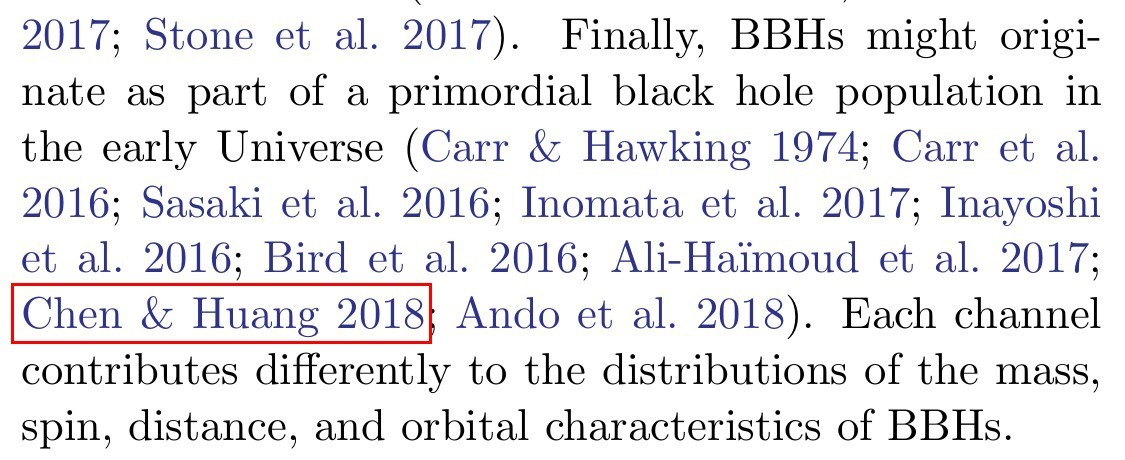
\includegraphics[width=0.7\textwidth]{./pic/ligocite02.jpg}
	\end{center}
%	\vspace{-3mm}

	\item \blue{Stochastic Gravitational-Wave Background from Binary Black Holes and Binary Neutron Stars and Implications for LISA} \\
	Astrophys. J. 871 (2019) no.1, 97\\
	\textbf{Zu-Cheng Chen}, Fan Huang, and Qing-Guo Huang
\end{enumerate} 
\end{frame}
%%%%%%%%%%%%%%%%%%%%%%%%%%%%%%%%%%%%%%%%%%%%%%%%%%%%%%%%%%%%%%%%%%%%%%%%%%%%%%%%

%%%%%%%%%%%%%%%%%%%%%%%%%%%%%%%%%%%%%%%%%%%%%%%%%%%%%%%%%%%%%%%%%%%%%%%%%%%%%%%%
\begin{frame}{科研文章}
    \begin{enumerate}[<+->]    
    \setcounter{enumi}{2}
    \item \blue{Distinguishing Primordial Black Holes from Astrophysical Black Holes by Einstein Telescope and Cosmic Explorer}\\ 
    arXiv:1904.02396\\
    \textbf{Zu-Cheng Chen}, and Qing-Guo Huang
    \vspace{2mm}
    
    \item \blue{Probing Primordial-Black-Hole Dark Matter with Scalar Induced Gravitational Waves}\\
    Phys. Rev. D100 (2019) 081301 [Rapid Communications]\\
    Chen Yuan, \textbf{Zu-Cheng Chen}, and Qing-Guo Huang, "
    \vspace{2mm}
     
    \item \blue{Measuring the tilt of primordial gravitational-wave power spectrum from observations}\\
    Sci. China Phys. Mech. Astron. 62 (2019) no.11, 110421\\
    Jun Li, \textbf{Zu-Cheng Chen}, and Qing-Guo Huang
    \vspace{2mm}
\end{enumerate} 
\end{frame}
%%%%%%%%%%%%%%%%%%%%%%%%%%%%%%%%%%%%%%%%%%%%%%%%%%%%%%%%%%%%%%%%%%%%%%%%%%%%%%%%

%%%%%%%%%%%%%%%%%%%%%%%%%%%%%%%%%%%%%%%%%%%%%%%%%%%%%%%%%%%%%%%%%%%%%%%%%%%%%%%%
\begin{frame}{科研文章}
    \begin{enumerate}[<+->]    
    \setcounter{enumi}{5}    
    \item \blue{Extraction of gravitational wave signals with optimized convolutional neural network}\\
    Frontiers of Physics [accepted]\\
    Hua-Mei Luo, Wenbin Lin, \textbf{Zu-Cheng Chen}, and Qing-Guo Huang
    \vspace{2mm}
    
    \item \blue{Log-dependent slope of scalar induced gravitational waves in the infrared regions}\\
    arXiv:1910.09099 \\
    Chen Yuan, \textbf{Zu-Cheng Chen}, and Qing-Guo Huang
    \vspace{2mm}
    
    \item \blue{Pulsar Timing Array Constraints on Primordial Black Holes with NANOGrav 11-Year Data Set}\\
    arXiv:1910.12239 \\
    \textbf{Zu-Cheng Chen}, Chen Yuan, and Qing-Guo Huang
\end{enumerate} 
\end{frame}

\section{开源项目}
%%%%%%%%%%%%%%%%%%%%%%%%%%%%%%%%%%%%%%%%%%%%%%%%%%%%%%%%%%%%%%%%%%%%%%%%%%%%%%%%
\subsection{}
%%%%%%%%%%%%%%%%%%%%%%%%%%%%%%%%%%%%%%%%%%%%%%%%%%%%%%%%%%%%%%%%%%%%%%%%%%%%%%%%
\begin{frame}{开源项目}
    \vspace{-2mm}
    \begin{enumerate}
        \item 发起\blue{《引力波数据分析入门》}维基教科书项目。
        \begin{figure}[htbp!]
            \centering
            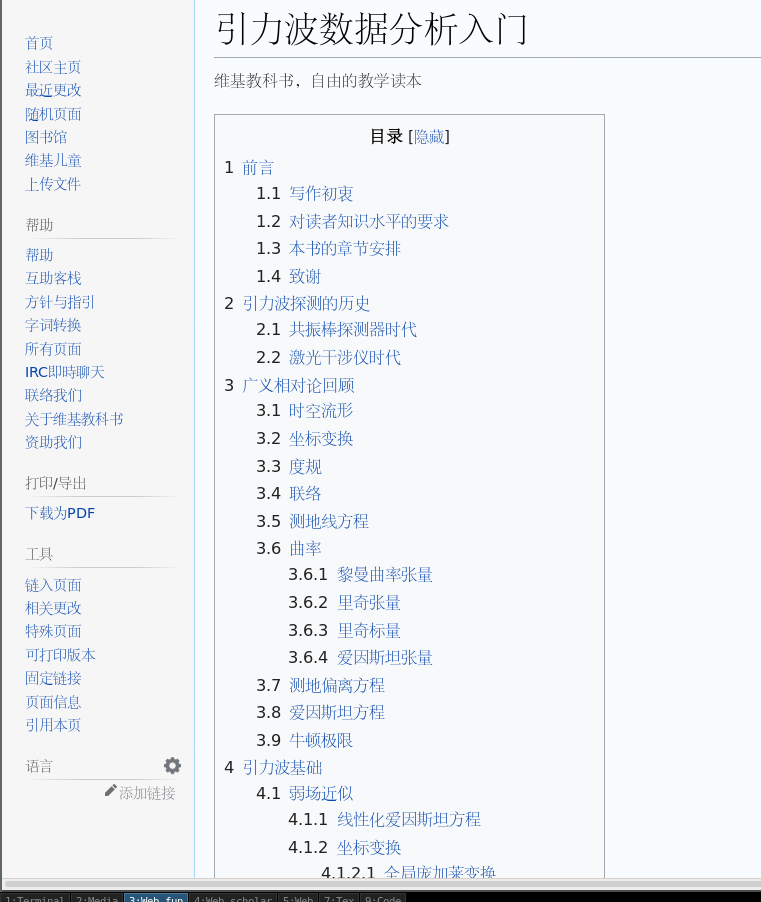
\includegraphics[width = 0.65\textwidth]{./pic/GW_book.png}
        \end{figure}
    \end{enumerate} 
\end{frame}

%%%%%%%%%%%%%%%%%%%%%%%%%%%%%%%%%%%%%%%%%%%%%%%%%%%%%%%%%%%%%%%%%%%%%%%%%%%%%%%%
\begin{frame}{开源项目}
    \vspace{-2mm}
    \begin{enumerate}        
    \setcounter{enumi}{1}
        \item \texttt{PSO.jl}:用julia语言实现了粒子群优化算法
        \begin{figure}[htbp!]
            \centering
            \includegraphics[width = 0.75\textwidth]{./pic/PSO.png}
        \end{figure}
    \end{enumerate} 
\end{frame}

%%%%%%%%%%%%%%%%%%%%%%%%%%%%%%%%%%%%%%%%%%%%%%%%%%%%%%%%%%%%%%%%%%%%%%%%%%%%%%%%
\begin{frame}{开源项目}
    \vspace{-2mm}
    \begin{enumerate}
    \setcounter{enumi}{2}     
        \item \texttt{GWSC.jl}:用julia语言实现了计算引力波灵敏度曲线的程序
        \begin{figure}[htbp!]
            \centering
            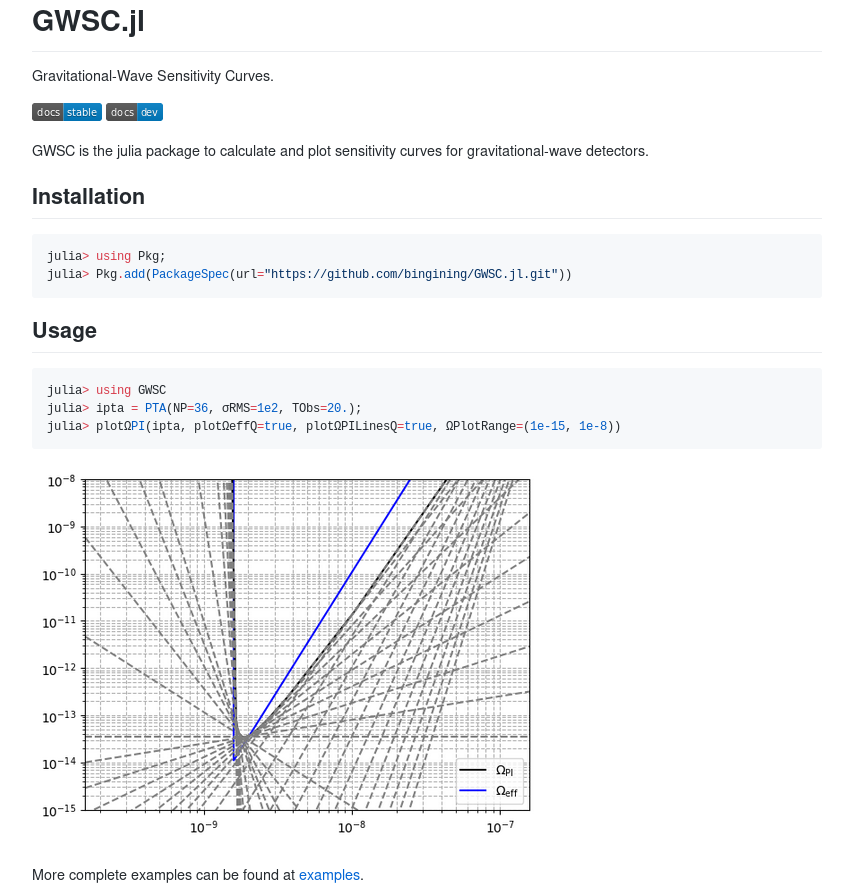
\includegraphics[width = 0.75\textwidth]{./pic/GWSC.png}
        \end{figure}
    \end{enumerate} 
\end{frame}

\section{团学会活动}
%%%%%%%%%%%%%%%%%%%%%%%%%%%%%%%%%%%%%%%%%%%%%%%%%%%%%%%%%%%%%%%%%%%%%%%%%%%%%%%%
\subsection{}
%%%%%%%%%%%%%%%%%%%%%%%%%%%%%%%%%%%%%%%%%%%%%%%%%%%%%%%%%%%%%%%%%%%%%%%%%%%%%%%%
\begin{frame}{团学会活动}
    \begin{enumerate}[<+->]   
        \item 担任2019年度\blue{体育部部长}
        \vspace{2mm}
        
        \item 2019年研究生及博士后\blue{新年联欢会}
        \vspace{2mm}
        
        \item 理论物理所第十一届\blue{乒乓球友谊赛}
        \vspace{2mm}
        
        \item 中科院北京分院首届职工田径运动会开幕式\blue{广播操展示}
    \end{enumerate} 
\end{frame}

\section{获奖情况}
%%%%%%%%%%%%%%%%%%%%%%%%%%%%%%%%%%%%%%%%%%%%%%%%%%%%%%%%%%%%%%%%%%%%%%%%%%%%%%%%
\subsection{}
%%%%%%%%%%%%%%%%%%%%%%%%%%%%%%%%%%%%%%%%%%%%%%%%%%%%%%%%%%%%%%%%%%%%%%%%%%%%%%%%
\begin{frame}{获奖情况}
    \begin{enumerate}[<+->]   
        \item 2018年获得\blue{曙光特别奖}
        \vspace{2mm}
        \item 2019年获得中国科学院大学\blue{三好学生}称号
    \end{enumerate} 
\end{frame}

%%%%%%%%%%%%%%%%%%%%%%%%%%%%%%%%%%%%%%%%%%%%%%%%%%%%%%%%%%%%%%%%%%%%%%%%%%%%%%%%
%\section{Introduction}
\section{典型成果}
%%%%%%%%%%%%%%%%%%%%%%%%%%%%%%%%%%%%%%%%%%%%%%%%%%%%%%%%%%%%%%%%%%%%%%%%%%%%%%%%
%%%%%%%%%%%%%%%%%%%%%%%%%%%%%%%%%%%%%%%%%%%%%%%%%%%%%%%%%%%%%%%%%%%%%%%%%%%%%%%%
\subsection{}

%%%%%%%%%%%%%%%%%%%%%%%%%%%%%%%%%%%%%%%%%%%%%%%%%%%%%%%%%%%%%%%%%%%%%%%%%%%%%%%%
%\begin{frame}{Scalar induced gravitational wave up to $3$rd order}
%    \be
%    \rd s^{2}=a^{2}\left\{-(1+2 \phi) \rd \eta^{2}+\left[(1-2 \phi) \delta_{i j}+\frac{h_{i j}}{2}\right] \rd x^{i} \rd x^{j}\right\},
%    \ee
%    
%    \be
%    h_{i j}^{\prime \prime}+2 \mathcal{H} h_{i j}^{\prime}-\nabla^{2} h_{i j}=-4 \mathcal{T}_{i j}^{\ell m} S_{\ell m},
%    \ee
%\end{frame}
%%%%%%%%%%%%%%%%%%%%%%%%%%%%%%%%%%%%%%%%%%%%%%%%%%%%%%%%%%%%%%%%%%%%%%%%%%%%%%%%
%%%%%%%%%%%%%%%%%%%%%%%%%%%%%%%%%%%%%%%%%%%%%%%%%%%%%%%%%%%%%%%%%%%%%%%%%%%%%%%%
\begin{frame}{典型成果 (合作者:黄庆国、袁晨)}    
    \begin{itemize}
        \item \blue{Probing Primordial-Black-Hole Dark Matter with Scalar Induced Gravitational Waves}\\
        Phys. Rev. D100 (2019) 081301 [Rapid Communications]\\
        Chen Yuan, \textbf{Zu-Cheng Chen}, and Qing-Guo Huang, "
        \vspace{2mm}
        
        \item \blue{Pulsar Timing Array Constraints on Primordial Black Holes with NANOGrav 11-Year Data Set}\\
        arXiv:1910.12239 \\
        \textbf{Zu-Cheng Chen}, Chen Yuan, and Qing-Guo Huang
    \end{itemize}
\end{frame}
%%%%%%%%%%%%%%%%%%%%%%%%%%%%%%%%%%%%%%%%%%%%%%%%%%%%%%%%%%%%%%%%%%%%%%%%%%%%%%%%

%%%%%%%%%%%%%%%%%%%%%%%%%%%%%%%%%%%%%%%%%%%%%%%%%%%%%%%%%%%%%%%%%%%%%%%%%%%%%%%%
\begin{frame}{标量诱导的次生引力波的$3$阶修正}	
%    \vspace{-1.5mm} 
%    \centering
%    \small{\textit{Done with Qing-Guo Huang and Chen Yuan.}}
    \vspace{-2.5mm}
    \begin{figure}[htbp!]
        \centering
        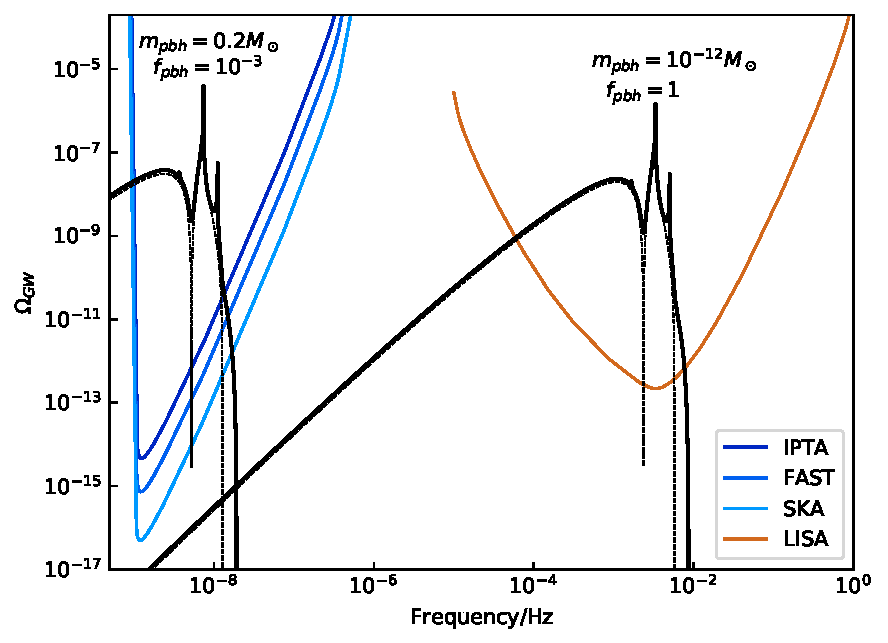
\includegraphics[width = \textwidth]{./pic/OmegaGW.pdf}
    \end{figure}
\end{frame}
%%%%%%%%%%%%%%%%%%%%%%%%%%%%%%%%%%%%%%%%%%%%%%%%%%%%%%%%%%%%%%%%%%%%%%%%%%%%%%%%

%%%%%%%%%%%%%%%%%%%%%%%%%%%%%%%%%%%%%%%%%%%%%%%%%%%%%%%%%%%%%%%%%%%%%%%%%%%%%%%%
\begin{frame}{标量诱导的次生引力波的$3$阶修正}
    \vspace{-2.5mm} 
\begin{figure}[htbp!]
    \centering
    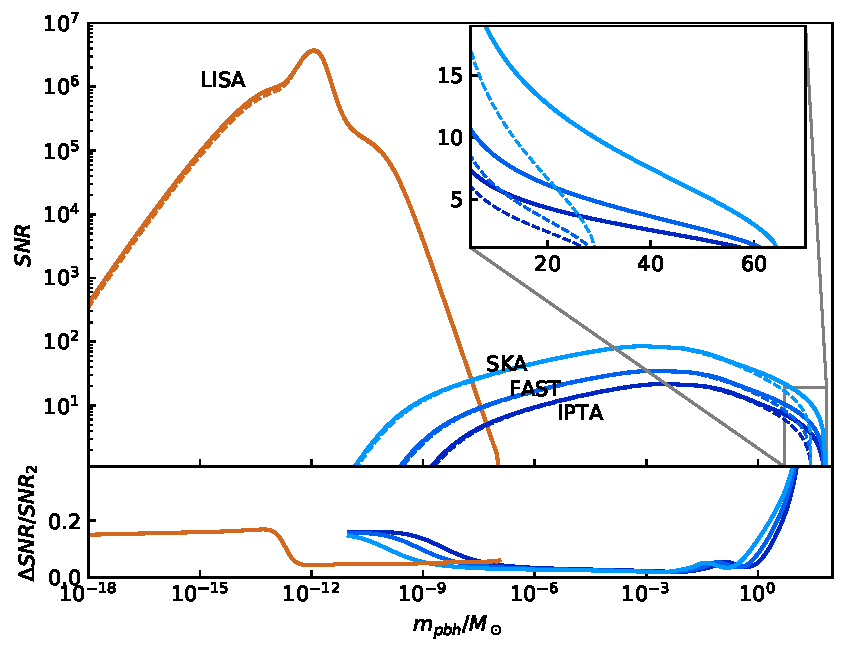
\includegraphics[width = 0.95\textwidth]{./pic/SNR.pdf}
\end{figure}
\end{frame}
%%%%%%%%%%%%%%%%%%%%%%%%%%%%%%%%%%%%%%%%%%%%%%%%%%%%%%%%%%%%%%%%%%%%%%%%%%%%%%%%

%%%%%%%%%%%%%%%%%%%%%%%%%%%%%%%%%%%%%%%%%%%%%%%%%%%%%%%%%%%%%%%%%%%%%%%%%%%%%%%%
\begin{frame}{NANOGrav数据对原初黑洞的限制}
    \vspace{-1.5mm} 
    \centering
    $A$: 标量扰动功率谱的振幅
    \vspace{-1.0mm} 
    \begin{figure}[htbp!]
        \centering
        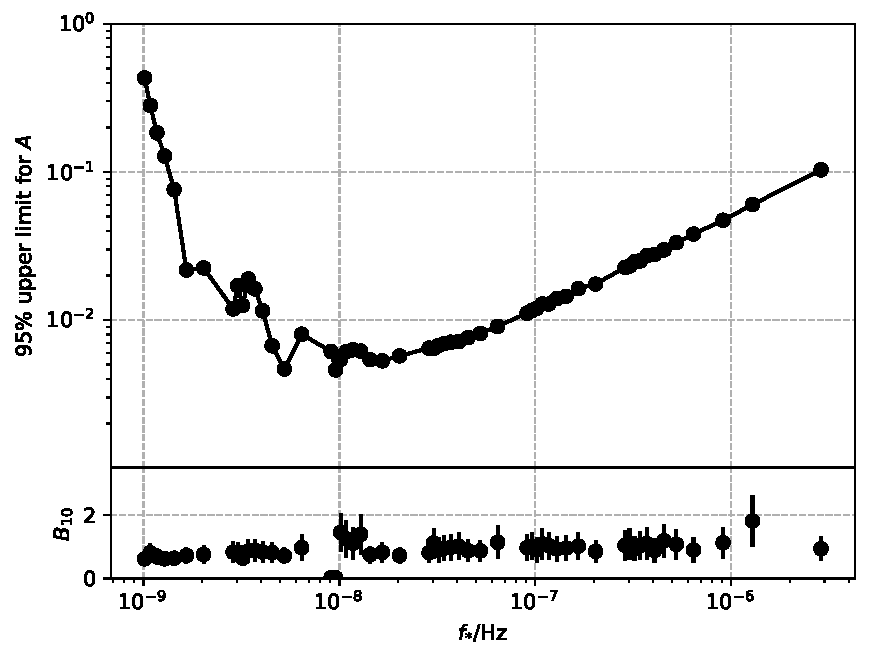
\includegraphics[width = 0.88\textwidth]{./pic/A_upper.pdf}
    \end{figure}
\end{frame}
%%%%%%%%%%%%%%%%%%%%%%%%%%%%%%%%%%%%%%%%%%%%%%%%%%%%%%%%%%%%%%%%%%%%%%%%%%%%%%%%

%%%%%%%%%%%%%%%%%%%%%%%%%%%%%%%%%%%%%%%%%%%%%%%%%%%%%%%%%%%%%%%%%%%%%%%%%%%%%%%%
\begin{frame}{NANOGrav数据对原初黑洞的限制}
    \vspace{-2.5mm} 
    \begin{figure}[htbp!]
        \centering
        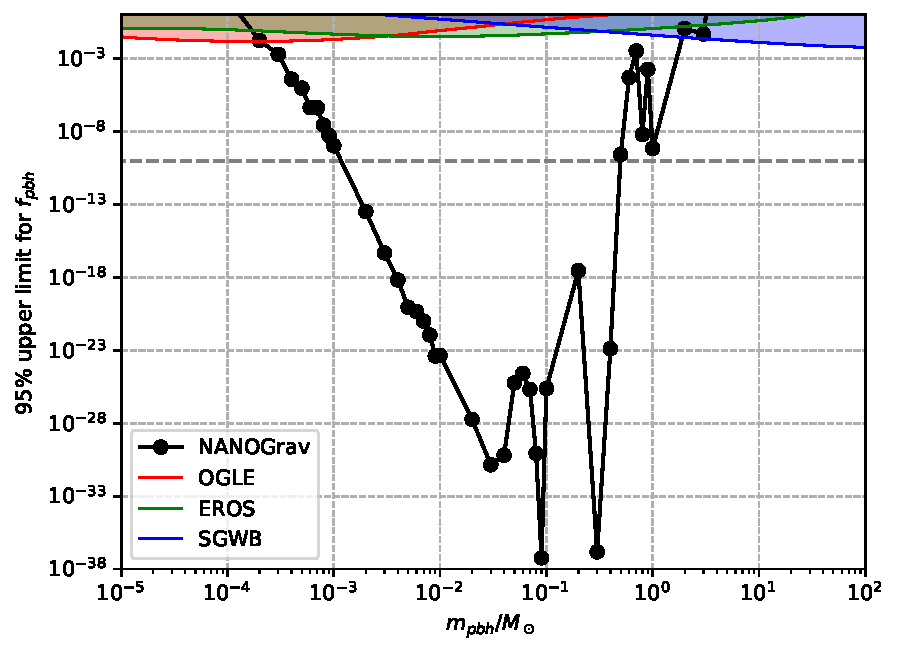
\includegraphics[width = \textwidth]{./pic/fpbh_upper.pdf}
    \end{figure}
\end{frame}
%%%%%%%%%%%%%%%%%%%%%%%%%%%%%%%%%%%%%%%%%%%%%%%%%%%%%%%%%%%%%%%%%%%%%%%%%%%%%%%%

%%%%%%%%%%%%%%%%%%%%%%%%%%%%%%%%%%%%%%%%%%%%%%%%%%%%%%%%%%%%%%%%%%%%%%%%%%%%%%%%
\begin{frame}{典型成果小结} 
\begin{itemize}
    \item 计算了伴随原初黑洞产生而产生的次生引力波的三阶修正。
    \vspace{2mm}\pause
        
    \item 用NANOGrav脉冲星计时阵列的数据限制了原初黑洞的丰度。 
\end{itemize} 
\pause
\begin{center}
    \font\endfont = cmss12 at 12mm
    \color{Blue}
    \endfont
    \baselineskip 20.0mm
    Thank You
\end{center} 
\end{frame}
%%%%%%%%%%%%%%%%%%%%%%%%%%%%%%%%%%%%%%%%%%%%%%%%%%%%%%%%%%%%%%%%%%%%%%%%%%%%%%%%



%%%%%%%%%%%%%%%%%%%%%%%%%%%%%%%%%%%%%%%%%%%%%%%%%%%%%%%%%%%%%%%%%%%%%%%%%%%%%%%%
\end{document}
